\subsection{Cut-off and Saturation Regions:}

\setcounter{equation}{0}

The circuit in Figure 5.2.0 it's the same that Figure 3.2.0, but this time we are going to proceed to make the respective calculations. \hfill 

\begin{figure}[H]
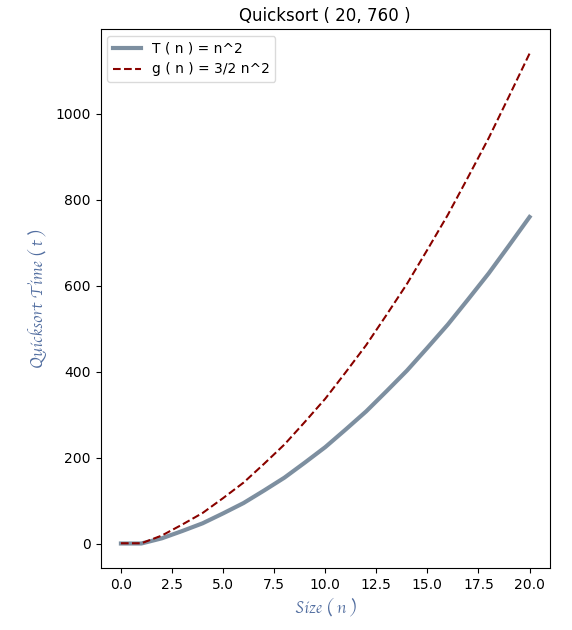
\includegraphics[scale=.6]{p2.png}
\centering \linebreak \linebreak Figure 5.2.0: Cut-off saturation points of a transistor.
\end{figure} \hfill 

{\bfseries\itshape
\begin{itemize}
\item Setting $V_{i}$ = 5 V Analysis, and using:
\begin{tasks}
\task $V_{BE} =  0.7 V$
\task $R_{C} = 100 \Omega$ 
\task $R_{B} = 10K \Omega$ 
\task $R_{E} = 0 \Omega$ 
\task $\beta = 242$ 
\end{tasks}
\end{itemize}} \hfill \break

{\bfseries\itshape\color{Violet}{
\begin{itemize}
\item For $I_{B}:$
\end{itemize}}} 

\begin{flushright}
{\bfseries\itshape\color{carmine}{Formula: $I_{B}\ =\ \frac{E_{B}\ -\ V_{BE}}{R_{B}\ +\ (\ \beta\ +\ 1\ )\ (\ R_{E}\ )}:$}} \hfill \break
\end{flushright}

\begin{ceqn}
\begin{align}
I_{B}\ &=\ \frac{5\ V\ -\ 0.7\ V}{10\ K\Omega\ +\ (\ \beta\ +\ 1\ )\ (\ 0\ \Omega\ )} \\ \\
&= 430 \mu A
\end{align}
\end{ceqn} \hfill \break

{\bfseries\itshape\color{Violet}{
\begin{itemize}
\item For $I_{C}:$
\end{itemize}}} 

\begin{flushright}
{\bfseries\itshape\color{carmine}{Formula: $I_{C}\ =\ (\ \beta\ )\ I_{B}:$}} \hfill \break
\end{flushright} \hfill

\begin{ceqn}
\begin{align}
I_{C}\ &=\ (\ 242\ )\ (\ 430\ \mu A\ ) \\ \\
&=\ 0.10\ A
\end{align}
\end{ceqn} \hfill \break

\pagebreak

{\bfseries\itshape\color{Violet}{
\begin{itemize}
\item For $V_{CE}:$
\end{itemize}}} 

\begin{flushright}
{\bfseries\itshape\color{carmine}{Formula: $V_{CE}\ =\ E_{C}\ -\ I_{C}\ (\ R_{C}\ +\ R_{E}\ ):$}} \hfill \break
\end{flushright}

\begin{ceqn}
\begin{align}
V_{CE}\ &=\ 12\ V\ -\ 0.10\ A\ (\ 100\ \Omega\ +\ 0\ \Omega\ ) \\ \\
&=\ 2 V
\end{align}
\end{ceqn} \hfill \break

\pagebreak

{\bfseries\itshape
\begin{itemize}
\item Setting $V_{i}$ = 0 V Analysis, and using:
\begin{tasks}
\task $V_{BE} =  0.7 V$
\task $R_{C} = 100 \Omega$ 
\task $R_{B} = 10K \Omega$ 
\task $R_{E} = 0 \Omega$ 
\task $\beta = 242$ 
\end{tasks}
\end{itemize}} \hfill \break

{\bfseries\itshape\color{Violet}{
\begin{itemize}
\item For $I_{B}:$
\end{itemize}}}

\begin{flushright}
{\bfseries\itshape\color{carmine}{Formula: $I_{B}\ =\ \frac{E_{B}\ -\ V_{BE}}{R_{B}\ +\ (\ \beta\ +\ 1\ )\ (\ R_{E}\ )}:$}} \hfill \break
\end{flushright}

\begin{ceqn}
\begin{align}
I_{B}\ &=\ \frac{0\ V\ -\ 0.7\ V}{10\ K\Omega\ +\ (\ \beta\ +\ 1\ )\ (\ 0\ \Omega\ )} \\ \\
&\cong 0 A
\end{align}
\end{ceqn} \hfill \break

{\bfseries\itshape\color{Violet}{
\begin{itemize}
\item For $I_{C}:$
\end{itemize}}} 

\begin{flushright}
{\bfseries\itshape\color{carmine}{Formula: $I_{C}\ =\ (\ \beta\ )\ I_{B}:$}} \hfill \break
\end{flushright}

\begin{ceqn}
\begin{align}
I_{C}\ &=\ (\ 242\ )\ (\ 0\ A\ ) \\ \\
&=\ 0\ A
\end{align}
\end{ceqn} \hfill \break

{\bfseries\itshape\color{Violet}{
\begin{itemize}
\item For $V_{CE}:$
\end{itemize}}} 

\begin{flushright}
{\bfseries\itshape\color{carmine}{Formula: $V_{CE}\ =\ E_{C}\ -\ I_{C}\ (\ R_{C}\ +\ R_{E}\ ):$}} \hfill \break
\end{flushright}

\begin{ceqn}
\begin{align}
V_{CE}\ &=\ 12\ V\ -\ 0\ A\ (\ 100\ \Omega\ +\ 0\ \Omega\ ) \\ \\
&=\ 12 V
\end{align}
\end{ceqn} \hfill \break

\pagebreak

The same process previously performed for calculating $I_{C},\ I_{B}, V_{CE}$ will be repeated bellow, the difference lays this time in the resistor $R_{B}$ that we will use. \hfill \break

{\bfseries\itshape
\begin{itemize}
\item Setting $V_{i}$ = 5 V Analysis, and using:
\begin{tasks}
\task $V_{BE} =  0.7 V$
\task $R_{C} = 100 \Omega$ 
\task $R_{B} = 22K \Omega$ 
\task $R_{E} = 0 \Omega$ 
\task $\beta = 242$ 
\end{tasks}
\end{itemize}} \hfill \break

{\bfseries\itshape\color{Violet}{
\begin{itemize}
\item For $I_{B}:$
\end{itemize}}} 

\begin{flushright}
{\bfseries\itshape\color{carmine}{Formula: $I_{B}\ =\ \frac{E_{B}\ -\ V_{BE}}{R_{B}\ +\ (\ \beta\ +\ 1\ )\ (\ R_{E}\ )}:$}} \hfill \break
\end{flushright}

\begin{ceqn}
\begin{align}
I_{B}\ &=\ \frac{5\ V\ -\ 0.7\ V}{22\ K\Omega\ +\ (\ \beta\ +\ 1\ )\ (\ 0\ \Omega\ )} \\ \\
&= 195 \mu A
\end{align}
\end{ceqn} \hfill \break

{\bfseries\itshape\color{Violet}{
\begin{itemize}
\item For $I_{C}:$
\end{itemize}}} 

\begin{flushright}
{\bfseries\itshape\color{carmine}{Formula: $I_{C}\ =\ (\ \beta\ )\ I_{B}:$}} \hfill \break
\end{flushright}

\begin{ceqn}
\begin{align}
I_{C}\ &=\ (\ 242\ )\ (\ 195\ \mu A\ ) \\ \\
&=\ 0.047\ A
\end{align}
\end{ceqn} \hfill \break

{\bfseries\itshape\color{Violet}{
\begin{itemize}
\item For $V_{CE}:$
\end{itemize}}} 

\begin{flushright}
{\bfseries\itshape\color{carmine}{Formula: $V_{CE}\ =\ E_{C}\ -\ I_{C}\ (\ R_{C}\ +\ R_{E}\ ):$}} \hfill \break
\end{flushright}

\begin{ceqn}
\begin{align}
V_{CE}\ &=\ 12\ V\ -\ 0.047\ A\ (\ 100\ \Omega\ +\ 0\ \Omega\ ) \\ \\
&=\ 7.2 V
\end{align}
\end{ceqn} \hfill \break

\pagebreak

{\bfseries\itshape
\begin{itemize}
\item Setting $V_{i}$ = 0 V Analysis, and using:
\begin{tasks}
\task $V_{BE} =  0.7 V$
\task $R_{C} = 100 \Omega$ 
\task $R_{B} = 22K \Omega$ 
\task $R_{E} = 0 \Omega$ 
\task $\beta = 242$ 
\end{tasks}
\end{itemize}} \hfill \break

{\bfseries\itshape\color{Violet}{
\begin{itemize}
\item For $I_{B}:$
\end{itemize}}} 

\begin{flushright}
{\bfseries\itshape\color{carmine}{Formula: $I_{B}\ =\ \frac{E_{B}\ -\ V_{BE}}{R_{B}\ +\ (\ \beta\ +\ 1\ )\ (\ R_{E}\ )}:$}} \hfill \break
\end{flushright}

\begin{ceqn}
\begin{align}
I_{B}\ &=\ \frac{0\ V\ -\ 0.7\ V}{22\ K\Omega\ +\ (\ \beta\ +\ 1\ )\ (\ 0\ \Omega\ )} \\ \\
&\cong 0 A
\end{align}
\end{ceqn} \hfill \break

{\bfseries\itshape\color{Violet}{
\begin{itemize}
\item For $I_{C}:$
\end{itemize}}} 

\begin{flushright}
{\bfseries\itshape\color{carmine}{Formula: $I_{C}\ =\ (\ \beta\ )\ I_{B}:$}} \hfill \break
\end{flushright}

\begin{ceqn}
\begin{align}
I_{C}\ &=\ (\ 242\ )\ (\ 0\ A\ ) \\ \\
&=\ 0\ A
\end{align}
\end{ceqn} \hfill \break

{\bfseries\itshape\color{Violet}{
\begin{itemize}
\item For $V_{CE}:$
\end{itemize}}}

\begin{flushright}
{\bfseries\itshape\color{carmine}{Formula: $V_{CE}\ =\ E_{C}\ -\ I_{C}\ (\ R_{C}\ +\ R_{E}\ ):$}} \hfill \break
\end{flushright}

\begin{ceqn}
\begin{align}
V_{CE}\ &=\ 12\ V\ -\ 0\ A\ (\ 100\ \Omega\ +\ 0\ \Omega\ ) \\ \\
&=\ 12 V
\end{align}
\end{ceqn} \hfill \break

\pagebreak